\chapter{Spannungsverteilung in luftgek"uhlten Transformatoren\label{chapter:thema}}
\lhead{Spannungsverteilung in luftgek"uhlten Transformatoren}
\begin{refsection}
\chapterauthor{Reto Christen}

\section{Einleitung}

Heutzutage werden elektronische Betriebsmittel mittels CAD-Programme berechnet und ausgelegt. Dies erm"oglicht eine einfache und kosteng"unstige Entwicklung sowie Herstellung, da der erste Prototyp die Erwartungen meistens bereits erf"ullt. Die L"osungen von CAD-Programmen, was nichts anderes als L"osungen von partiellen oder gew"ohnlichen Differentialgleichungen sind, ergeben neue Herausforderungen, wie beispielsweise in der Numerik. 

In diesem Kapitel wird ein solches Problem vorgestellt, genauer betrachtet und schlussendlich gel"ost.

\section{Problemstellung}

Luftgek"uhlte Transformatoren sind im Gegensatz zu "olgek"uhlten Transformatoren eher gef"ahrdet Teilentladungen oder gar Durchschl"age zu haben. Dies liegt daran, dass die Isolationsfestigkeit von Luft wesentlich schlechter als in Öl ist. Da ein luftgek"uhlter Transformator im Gegensatz zu einem "olgek"uhlten Transformator diverse Vorteile besitzt, ist es von Interesse, die elektrischen Felder so zu limitieren, damit Durchschl"age und gr"osstenteils auch Teilentladungen verhindert werden k"onnen. 

Fr"uher wurde ein Transformator oder allgemein ein elektronisches Betriebsmittel nach Erfahrungen gebaut. Dabei war es Gang und G"abe, dass es mehrere Prototypen brauchte, bis die ersten Spannungspr"ufungen bestanden werden konnten. Deshalb sind CAD-Simulationen wesentlich schneller und vor allem kosteng"unstiger. Das Ziel soll es sein, der Transformator m"oglichst genau darzustellen und dessen Spannungsverteilung zu berechnen, denn die Spannung und die Geometrie zusammen ergeben das elektrische Feld, welches schlussendlich zu Durchschl"agen oder Teilentladungen f"uhrt.

An der Hochschule f"ur Technik Rapperswil wurde am Institut f"ur Energietechnik eine Methode entwickelt, wie ein Blitzstoss Spannungsimpuls m"oglichst genau simuliert werden kann \cite{trafo:BILImpulse}. Dies Methode funktioniert sehr gut f"ur Leistungstransformatoren und konnte mit Messungen auch verifiziert werden. 
Will dieses Prinzip aber auf Instrumententransformatoren angewendet werden, ergibt die wesentlich h"ohere Anzahl von Wicklungen und deren engeren Lagen nummerische Probleme im L"osungsverfahren. 

Diese Probleme werden nun Schrittweise behandelt und bestm"oglich gel"ost. 


\subsection{Ersatzschaltbild}
Ein Transformator, ob "ol- oder luftgek"uhlt, kann prinzipiell mit dem Ersatzschaltbild \ref{trafo:einfaches_ESB} dargestellt werden. Dies macht Sinn, wenn der Transformator als Ganzes dargestellt werden will. Da bei diesem Problem aber die inneren Spannungen relevant sind, kann dieses bereits bekannte Ersatzschaltbild nicht verwendet werden. Es gilt nun, ein neues und genaueres Ersatzschaltbild zu finden. 

\begin{figure}
	\centering
	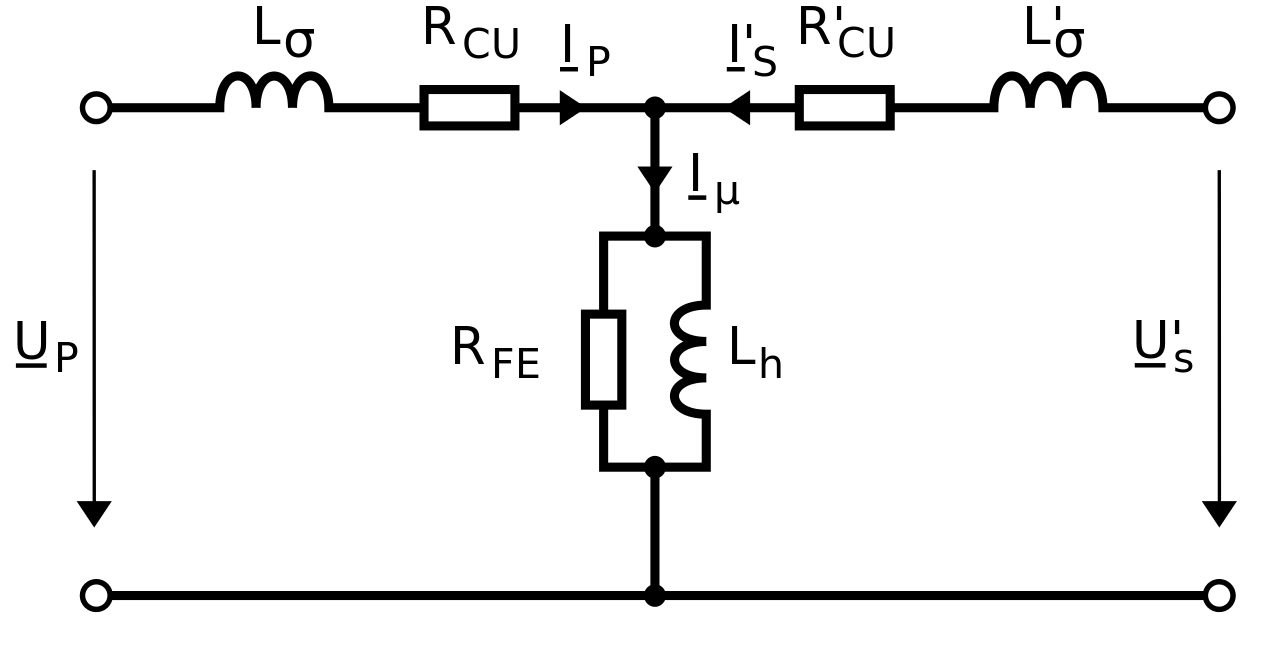
\includegraphics[width=0.5\textwidth]{./trafo/images/Einfaches_ESB.png}
	\caption[Einfach Ersatzschaltbild f"ur einen Transformator]{Einfach Ersatzschaltbild f"ur einen Transformator.}
	\label{trafo:einfaches_ESB}
\end{figure}

Ein Ansatz ist es, jede Wicklung einzeln zu modellieren. Pro Windung wird ein elektrischer Widerstand sowie Induktivit"at in Serie geschaltet. Ebenfalls m"ussen die Kapazit"aten sowie die Leitf"ahigkeiten gegen"uber Masse und den "ubrigen Windungen ber"ucksichtigt werden \cite{trafo:BILImpulse}. 

Dieses Ersatzschaltbild wird in der Abbildung \ref{trafo:erweitertes_ESB} dargestellt. Als Beispiel wird ein kleines Transformator Beispiel, bestehend aus 4 Windungen, verwendet. Mit Messungen an Testtransformatoren zeigte sich, das ab ca. 20 Windungen die Simulationen mit diesem Ersatzschaltbild sehr genau "ubereinstimmen. 

\begin{figure}
	\centering
	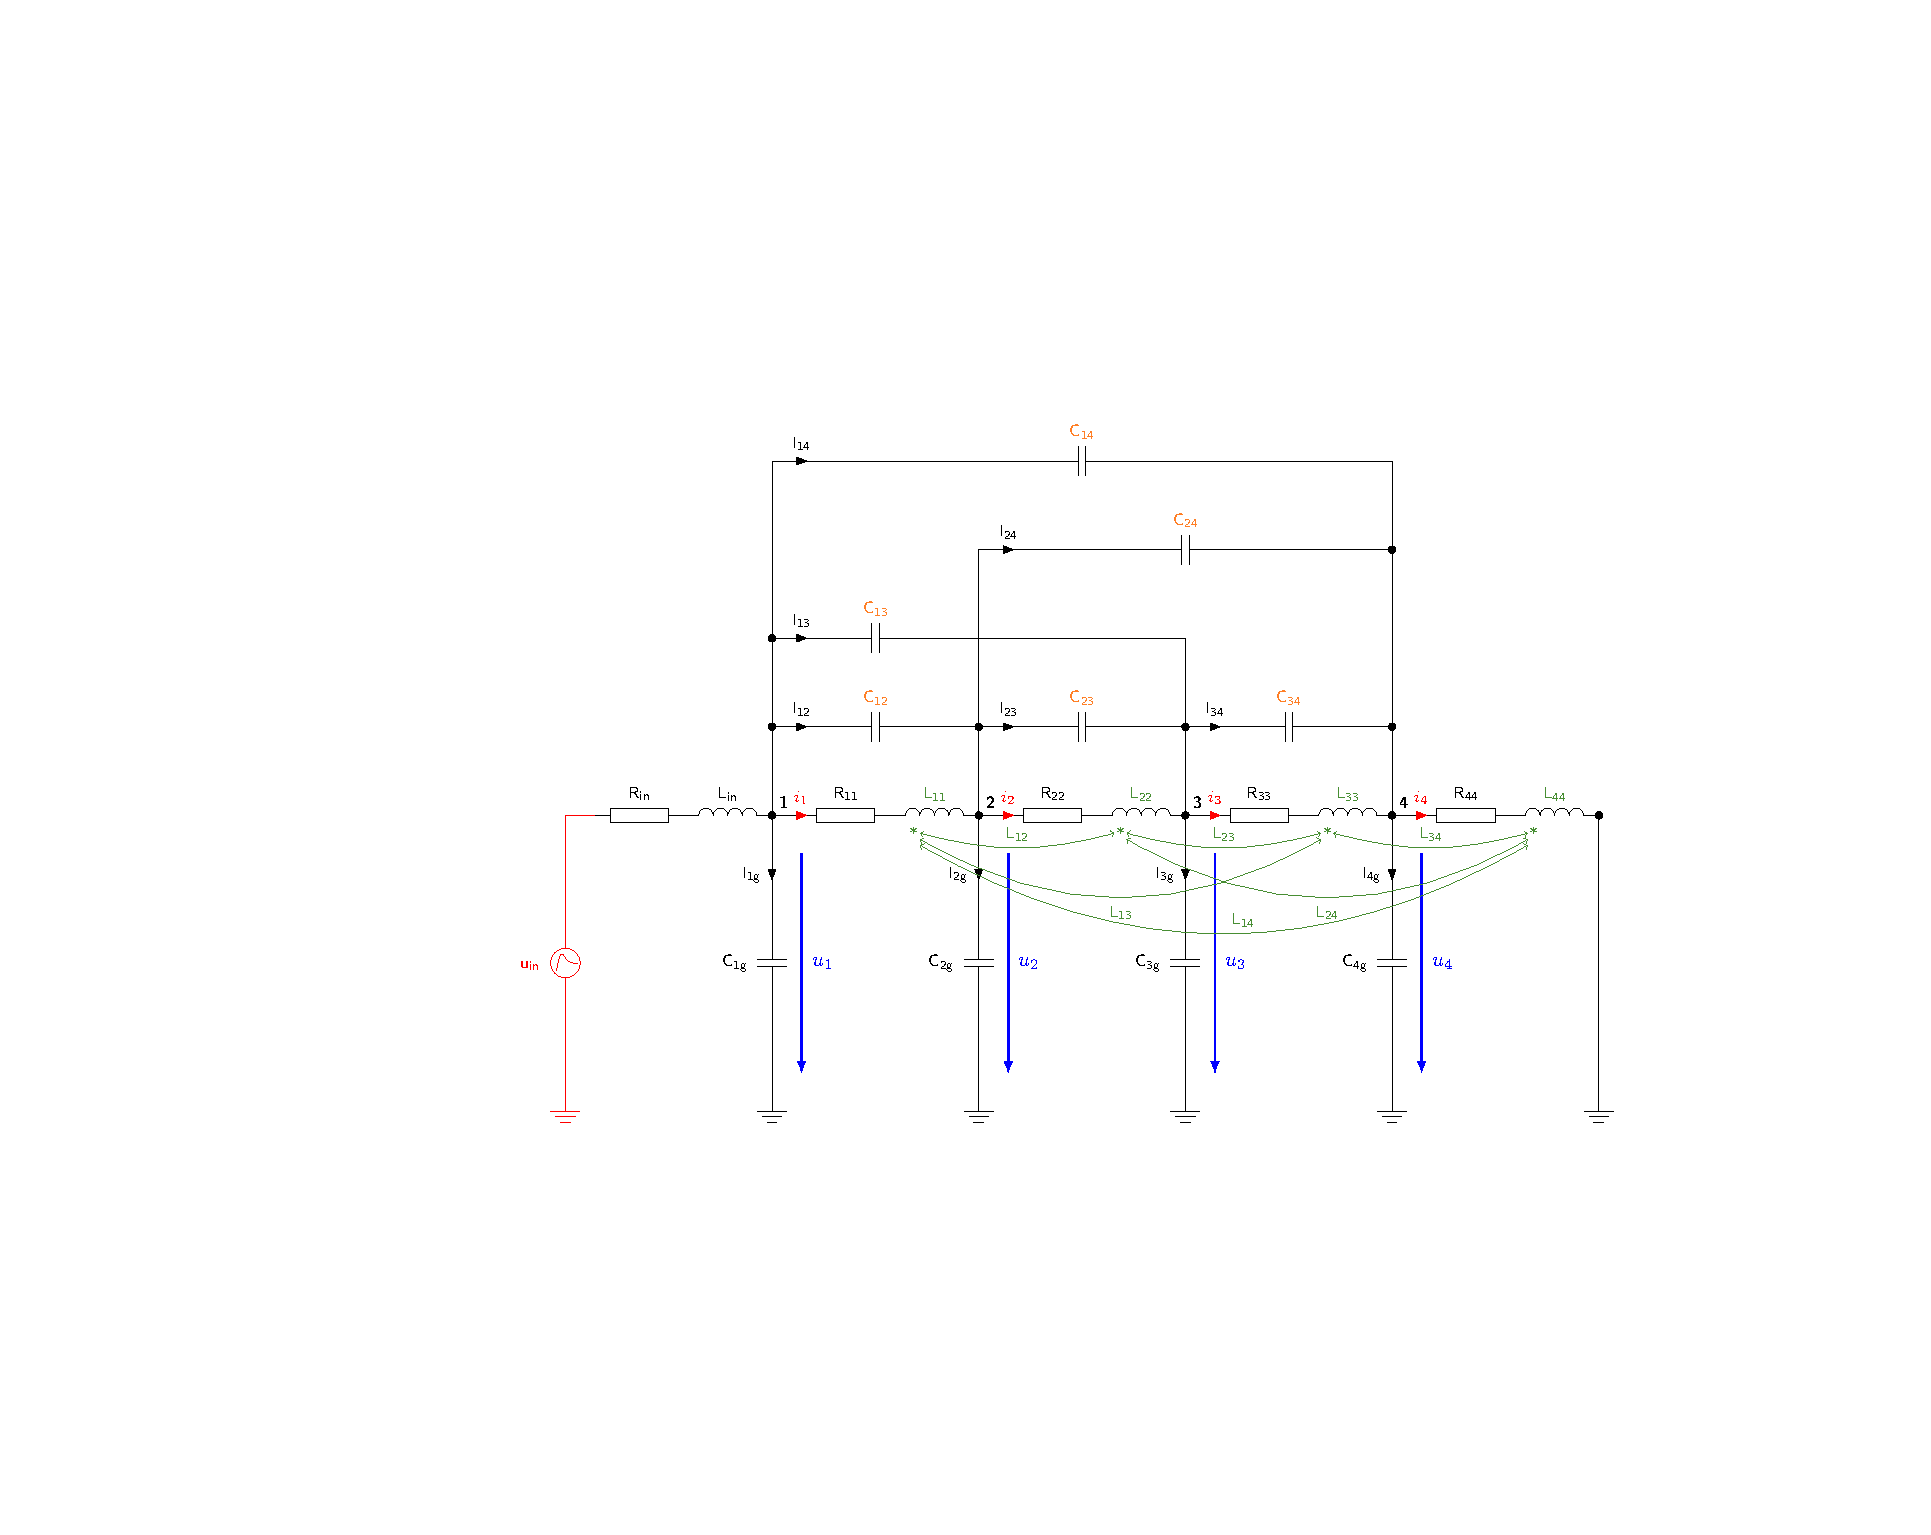
\includegraphics[width=0.8\textwidth]{./trafo/images/Trafo_Modell.pdf}
	\caption[Erweitertes Ersatzschaltbild f"ur einen Transformator]{Erweitertes Ersatzschaltbild f"ur einen Transformator mit 4 Wicklungen. Die Leitwerte zwischen den Wicklungen und gegen"uber Masse sind auf Grund der Übersichtlichkeit weggelassen worden. Die gr"unen Pfeile stellen die Mitkopplung der Spulen dar. }
	\label{trafo:erweitertes_ESB}
\end{figure}

Damit die Werte der einzelnen Elementen ermittelt werden k"onnen, sind Finite-Element-Methode-(FEM)-Simulationen in einem CAD Programm notwendig. Alle Wicklungen abgesehen einer werden auf das Spannungspotential \SI{0}{\volt} gesetzt. Die aktuelle gemessene Wicklung wird hingegen auf das Potential von \SI{1}{\volt} gesetzt und anschliessend werden die Induktivit"aten sowie Kapazit"aten gegen"uber allen anderen Wicklungen ermittelt.


\section{Mathematische L"osung}
\subsection{Differentialgleichung}

Es gilt nun eine Differentialgleichung f"ur das gefundene Ersatzschaltbild aufzustellen. Mittels dem Maschensatz (blaue Pfeile) und der Knotenpunktregel (rote Punkte) k"onnen die Differentialgleichungen pro Wicklung aufgestellt werden (dargestellt in \ref{trafo:orig}).

\begin{figure}
	\centering
	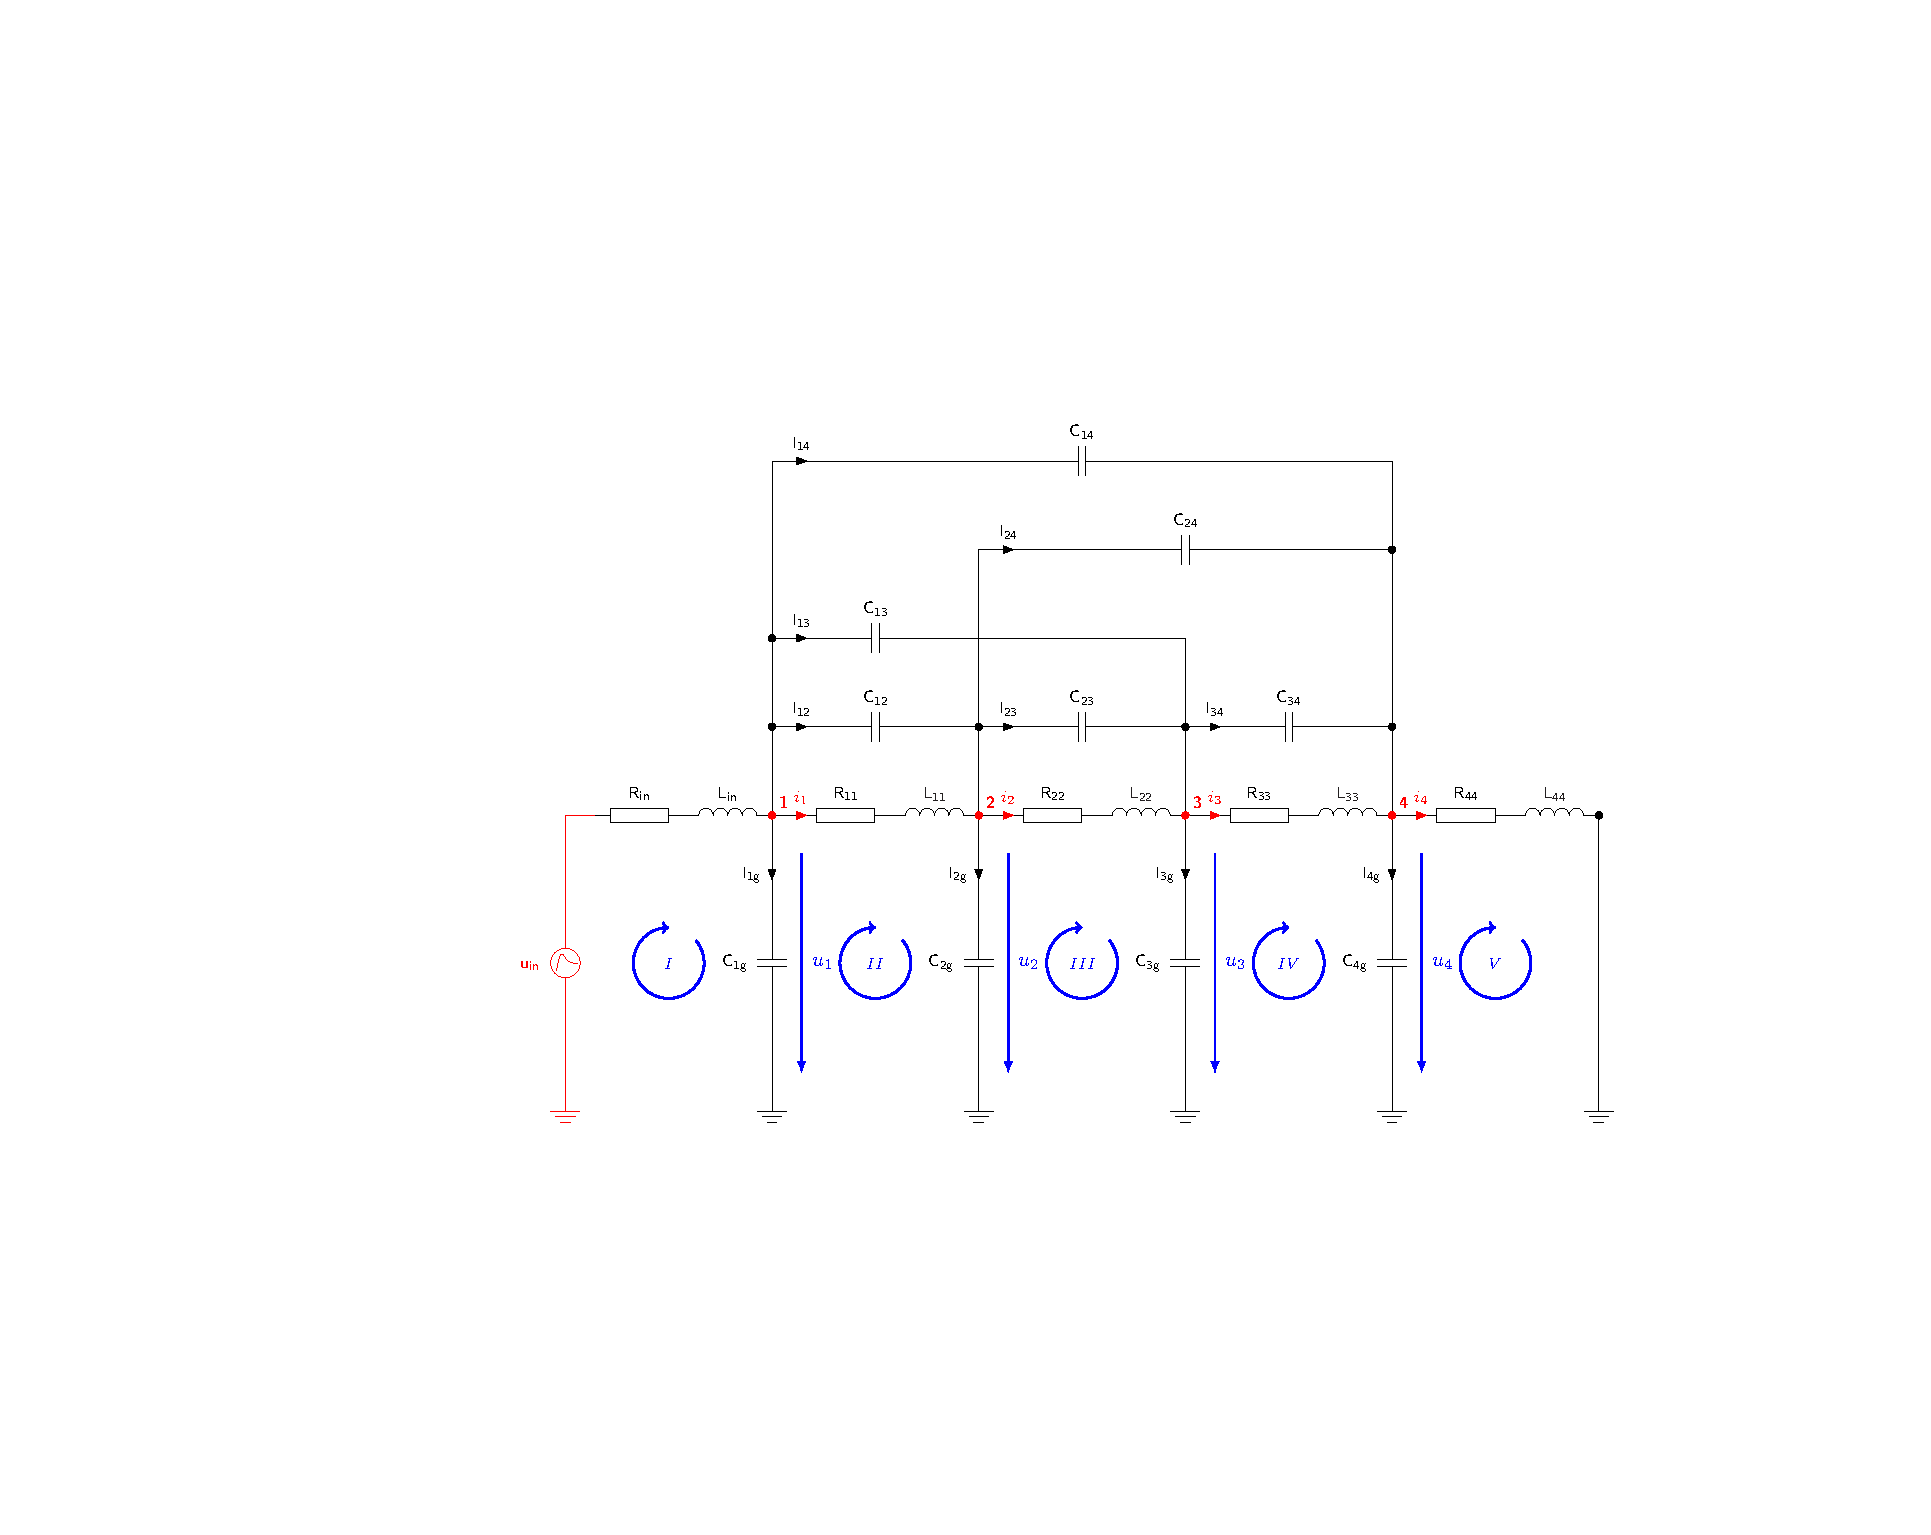
\includegraphics[width=0.8\textwidth]{./trafo/images/orig_trafo.pdf}
	\caption[Erweitertes Ersatzschaltbild f"ur einen Transformator mit Maschensatz und Knotenpunkt]{Erweitertes Ersatzschaltbild f"ur einen Transformator mit 4 Wicklungen. Die blaue Pfeilen stellen den Maschensatz und die roten Punkte den Knotenpunktregel dar.}
	\label{trafo:orig}
\end{figure}

Beispielsweise kann die Gleichungen der Wicklung 1 als 

\begin{equation*}
	u_\mathrm{Rin} + u_\mathrm{Lin} + u_1 = u_\mathrm{in}
\end{equation*}
und 
\begin{equation}
	i_\mathrm{in} = i_1 + i_{C1g} + i_{R12} + i_{C12} + i_{R13} + i_{C13} + i_{R14} + i_{C14}
\end{equation}
geschrieben werden. 

Mit etwas Umformungen kann der ganze Transformator als System mehreren Differentialgleichungen geschrieben werden \cite{trafo:SeminarCHR}. Als Beispiel wird wiederum der Transformator mit 4 Windungen gew"ahlt. Der Vektor $E$ ist der St"orterm, sprich in diesem Falle der Blitzstoss, des Systemes.

{\footnotesize 
\begin{align}
			&
			\underbrace{\begin{bmatrix}
			L_\mathrm{in}&0&0&0&0 & 0&0&0&0 \\
			0&L_{11}&L_{12}&L_{13}&L_{14} & 0&0&0&0 \\
			0&L_{21}&L_{22}&L_{23}&L_{24} & 0&0&0&0 \\
			0&L_{31}&L_{32}&L_{33}&L_{34} & 0&0&0&0 \\
			0&L_{41}&L_{42}&L_{43}&L_{44} & 0&0&0&0 \\
			0&0&0&0&0 & \sum{C_{1x}}&-C_{12}&-C_{13}&-C_{14} \\
			0&0&0&0&0 & -C_{21}&\sum{C_{2x}}&-C_{23}&-C_{24} \\
			0&0&0&0&0 & -C_{31}&-C_{32}&\sum{C_{3x}}&-C_{34} \\
			0&0&0&0&0 & -C_{41}&-C_{42}&-C_{43}&\sum{C_{4x}}
			    \end{bmatrix}}_{\text{$M$}}
			\cdot
			\underbrace{\begin{bmatrix}
			\frac{di_\mathrm{in}}{dt} \\
			\frac{di_1}{dt} \\
			\frac{di_2}{dt} \\
			\frac{di_3}{dt} \\
			\frac{di_4}{dt} \\
			\frac{du_1}{dt} \\
			\frac{du_2}{dt} \\
			\frac{du_3}{dt} \\
			\frac{du_4}{dt}
			\end{bmatrix}}_{\text{$\dot{x}$}}
			= \nonumber \\
			&
			\underbrace{\begin{bmatrix}
			-R_\mathrm{in}&0&0&0&0 & -1&0&0&0 \\
			0&-R_{11}&0&0&0 & 1&-1&0&0 \\
			0&0&-R_{22}&0&0 & 0&1&-1&0 \\
			0&0&0&-R_{33}&0 & 0&0&1&-1 \\
			0&0&0&0&-R_{44} & 0&0&0&1 \\
			1&-1&0&0&0 & -\sum G_{1x}&G_{12}&G_{13}&G_{14} \\
			0&1&-1&0&0 & G_{21} &- \sum G_{2x}& G_{23}& G_{24} \\
			0&0&1&-1&0 & G_{31} & G_{32} &-\sum G_{3x}&G_{34} \\
			0&0&0&1&-1 & G_{41}&G_{42}&G_{43}&-\sum G_{4x}
			\end{bmatrix}}_{\text{$F$}}
			\cdot
			\underbrace{\begin{bmatrix}
			i_\mathrm{in} \\
			i_1 \\
			i_2 \\
			i_3 \\
			i_4 \\
			u_1 \\
			u_2 \\
			u_3 \\
			u_4
			\end{bmatrix}}_{\text{$x$}}
			+
			\underbrace{\begin{bmatrix}
			u_\mathrm{in} \\
			0 \\
			0 \\
			0 \\
			0 \\
			0 \\
			0 \\
			0 \\
			0
			\end{bmatrix}}_{\text{$E$}}
			\label{trafo:DGL}
\end{align}
}
		


Die Matrix $M$ ist eine symmetrische Matrix, welches f"ur weitere Berechnungen wesentliche Vorteile mit sich bringt. Die Matrix $N$ ist fast symmetrisch. Wenn der Maschensatz jedoch in die andere Richtung wie in Abbildung \ref{trafo:orig} angewendet wird, l"asst sich auch diese Matrix mit fast keinem Aufwand symmetrisch machen. Dies ist f"ur dieses Beispiel zwar nicht n"otig, trotzdem kann es f"ur andere L"osungsans"atze von Vorteil sein. Aus der Gleichung \ref{trafo:DGL} wird nun 

{\footnotesize 
\begin{align}
			&
			\underbrace{\begin{bmatrix}
			\color{red}-\color{black}L_\mathrm{in}&0&0&0&0 & 0&0&0&0 \\
			0&\color{red}-\color{black}L_{11}&\color{red}-\color{black}L_{12}&\color{red}-\color{black}L_{13}&\color{red}-\color{black}L_{14} & 0&0&0&0 \\
			0&\color{red}-\color{black}L_{21}&\color{red}-\color{black}L_{22}&\color{red}-\color{black}L_{23}&\color{red}-\color{black}L_{24} & 0&0&0&0 \\
			0&\color{red}-\color{black}L_{31}&\color{red}-\color{black}L_{32}&\color{red}-\color{black}L_{33}&\color{red}-\color{black}L_{34} & 0&0&0&0 \\
			0&\color{red}-\color{black}L_{41}&\color{red}-\color{black}L_{42}&\color{red}-\color{black}L_{43}&\color{red}-\color{black}L_{44} & 0&0&0&0 \\
			0&0&0&0&0 & \sum{C_{1x}}&-C_{12}&-C_{13}&-C_{14} \\
			0&0&0&0&0 & -C_{21}&\sum{C_{2x}}&-C_{23}&-C_{24} \\
			0&0&0&0&0 & -C_{31}&-C_{32}&\sum{C_{3x}}&-C_{34} \\
			0&0&0&0&0 & -C_{41}&-C_{42}&-C_{43}&\sum{C_{4x}}
			    \end{bmatrix}}_{\text{$M$}}
			\cdot
			\underbrace{\begin{bmatrix}
			\frac{di_\mathrm{in}}{dt} \\
			\frac{di_1}{dt} \\
			\frac{di_2}{dt} \\
			\frac{di_3}{dt} \\
			\frac{di_4}{dt} \\
			\frac{du_1}{dt} \\
			\frac{du_2}{dt} \\
			\frac{du_3}{dt} \\
			\frac{du_4}{dt}
			\end{bmatrix}}_{\text{$\dot{x}$}}
			= \nonumber \\
			&
			\underbrace{\begin{bmatrix}
			\color{red}+\color{black}R_\mathrm{in}&0&0&0&0 & \color{red}+\color{black}1&0&0&0 \\
			0&\color{red}+\color{black}R_{11}&0&0&0 & \color{red}-\color{black}1&\color{red}+\color{black}1&0&0 \\
			0&0&\color{red}+\color{black}R_{22}&0&0 & 0&\color{red}-\color{black}1&\color{red}+\color{black}1&0 \\
			0&0&0&\color{red}+\color{black}R_{33}&0 & 0&0&\color{red}-\color{black}1&\color{red}+\color{black}1 \\
			0&0&0&0&\color{red}+\color{black}R_{44} & 0&0&0&\color{red}-\color{black}1 \\
			1&-1&0&0&0 & -\sum G_{1x}&G_{12}&G_{13}&G_{14} \\
			0&1&-1&0&0 & G_{21} &- \sum G_{2x}& G_{23}& G_{24} \\
			0&0&1&-1&0 & G_{31} & G_{32} &-\sum G_{3x}&G_{34} \\
			0&0&0&1&-1 & G_{41}&G_{42}&G_{43}&-\sum G_{4x}
			\end{bmatrix}}_{\text{$N$}}
			\cdot
			\underbrace{\begin{bmatrix}
			i_\mathrm{in} \\
			i_1 \\
			i_2 \\
			i_3 \\
			i_4 \\
			u_1 \\
			u_2 \\
			u_3 \\
			u_4
			\end{bmatrix}}_{\text{$x$}}
			+
			\underbrace{\begin{bmatrix}
			u_\mathrm{in} \\
			0 \\
			0 \\
			0 \\
			0 \\
			0 \\
			0 \\
			0 \\
			0
			\end{bmatrix}}_{\text{$E$}}
			\label{trafo:symmetricalDGL}
\end{align}
}

Dieses System mehrere Differentialgleichungen kann auch mit Matrizen und Vektoren geschrieben werden, welches sich etwas "ubersichtlicher darstellen l"asst. 

\begin{equation}
	M \cdot \dot x = N \cdot x + E
	\label{trafo:matricesDGL}
\end{equation}

Wird die Massenmatrix $M$ auf die rechte Seite der Gleichung \ref{trafo:matricesDGL} dividiert, ergibt dies

\begin{equation}
	\dot{x} = M^{-1} \cdot N \cdot x + M^{-1} \cdot E = A \cdot x + B
\end{equation}
welches die allgemein bekannte und auch l"osbare Zustandsraumdarstellung \index{Zustandsraumdarstellung} ist (engl. state space).

Das Problem scheint bereits gel"ost zu sein, insofern sich die Massenmatrix $M$ invertieren l"asst. In der Theorie w"are dies tats"achlich auch machbar, jedoch sehr aufw"andig. Weil auch gewisse Eigenwerte zu klein sind, explodiert die L"osung und kann somit mit diesem Ansatz nicht gel"ost werden.

Folglich muss ein Ansatz gefunden werden, welcher die Massenmatrix $M$ m"oglichst Rechenzeit-schonend invertiert und die Eigenwerte der Inversion im Griff hat. 


\subsection{Singular Value Decomposition (SVD) \index{Singular Value Decomposition}}
Eine M"oglichkeit stellt die Singular Value Decomposition, auf Deutsch Singul"arwertzerlegung, dar. Ohne Gedanken "uber die Dimensionen der Matrix $M$ zu verlieren, wird der SVD-Satz verwendet \cite{trafo:Watkins}. 

\begin{satz}
	\label{trafo:SVDTheorem}
	(\textit{SVD Theorem}) Sei $M\in \mathbb{R}^{n \times m}$ eine besetzte Matrix mit Rang $r$. Dann kann $M$ als Produkt von
	\begin{equation}
		M = USV^\top
		\label{trafo:svd}
	\end{equation} 
	geschrieben werden, wenn $U \in \mathbb{R}^{n \times n}$ und $V \in \mathbb{R}^{m \times m}$ orthogonal sind und $S \in \mathbb{R}^{n \times m}$ eine rechteckige Diagonalmatrix ist 
	\begin{equation*}
		S = \left( 
			\begin{array}{ccc|ccc}
				\lambda_1 &          &          &        & \vdots &        \\
				& \ddots   &          & \cdots & 0      & \cdots \\
				&          & \lambda_r &        & \vdots &        \\
				\hline
				&  \vdots  &          &        & \vdots &        \\
				\cdots   &  0       & \cdots   & \cdots & 0      & \cdots \\
				&  \vdots  &          &        & \vdots &   \\				
				\end{array}
			\right) 
			\hspace{2cm}\lambda_1 \geq \lambda_2 \geq \dots \lambda_r > 0. 
	\end{equation*}
\end{satz}
F"ur die Herleitung und den Beweis des Satzes \ref{trafo:SVDTheorem} wird auf die Fachliteratur verwiesen \cite{trafo:Watkins}.

Einfach erkl"aren l"asst sich die Singul"arwertzerlegung mit jeweils zwei Rotationen, es sind dies die Matrizen $U$ und $V^\top$, und einer Streckung durch die Diagonalmatrix $S$. Dieser Vorgang ist in Abbildung \ref{trafo:SVDFig} dargestellt. 

Die Matrix $U$ besitzt in der Senkrechte Eigenvektoren
\begin{equation*}
	\left( 
		\begin{array}{cccc}
		& & & \\
		u_1 & u_2 & \dots & u_n  \\
		& & & 			
		\end{array}
	\right) 
\end{equation*}
und lässt sich mit 
\begin{equation*}
	M M^\top = U S \underbrace{V^\top V}_{E} S^\top U^\top = U \underbrace{S S^\top}_{S^2} U
\end{equation*}
berechnen und anschliessend auflösen \cite{tafo:Watkins}.

Die Matrix $V$ besitzt in der Vertikale Eigenvektoren
\begin{equation*}
	\left( 
		\begin{array}{ccc}
		& v_1^\top & \\
		& v_2^\top & \\
		& \vdots & \\
		&  v_m^\top & \\			
		\end{array}
	\right) 
\end{equation*}
und lässt sich mit 
\begin{equation*}
	M^\top M = V S^\top \underbrace{U^\top U}_{E} S V^\top = V \underbrace{S^\top S}_{S^2} V^\top 
\end{equation*}
berechnen und anschliessend auflösen \cite{trafo:Watkins}.

Als etwas schnellere Alternative kann auch die Berechnung aus der Gleichung \ref{trafo:svd} erfolgen, denn $M$, $S$ und $U$ sind bekannt. 
\begin{align*}
	M^\top &= V \underbrace{S^\top}_{S} U^\top\\
	S^{-1} M^\top &= V U^\top\\
	V &= S^{-1} M^\top \left(U^\top\right) = S^{-1} M^\top U
\end{align*}

\begin{figure}
	\centering
	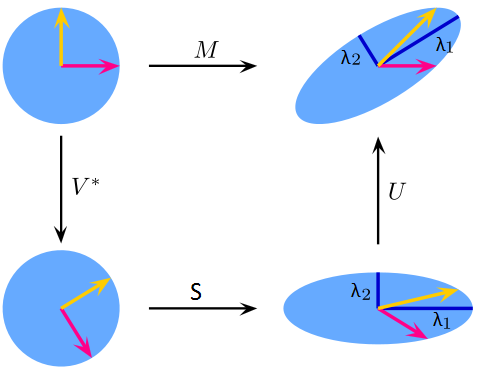
\includegraphics[width=0.6\textwidth]{./trafo/images/svd.png}
	\caption{Grafische Darstellung der Singul"arwertzerlegung \cite{trafo:SVDWiki}.}
	\label{trafo:SVDFig}
\end{figure}

Da es sich bei der Matrix $M$ um eine symmetrische Matrix handelt, sind die beiden Matrizen $U$ und $V$ im Betrag identisch. Falls die Eigenwerte der der Matrix $M$ alle dasselbe Vorzeichen besitzen, sind die Matrizen $U$ und $V$ gar identisch. Weil ein Transformator rein logisch gesehen unbedingt eine D"ampfung, sprich alle Eigenwerte negativ, haben muss, gilt $U = V$. Dies kann auch nummerisch verifiziert werden.

\subsubsection{Unterdrückung von unerwünschten Eigenwerte}
Die quadratische Diagonalmatrix $S$ wegen der symmetrischen Matrix $M$ zu einer quadratischen Matrix. Dies bedeutet, dass sich auf der ganzen Diagonale Eigenwerte des Systems befinden. Ein Ansatz zur Unterdr"uckung unerw"unschten Frequenzen kann sein, zu kleine Eigenwerte $\lambda < tol$, welche in der Numerik 'explodieren' und physisch gesehen zu grosse und unm"ogliche Frequenzen sind, auf Null zu setzen. Dies ergibt die Diagonalmatrix 
\begin{equation*}
	S = \left( 
			\begin{array}{cccccc}
				\lambda_1 & & & & & \\
				& \ddots & & & &  \\
				& & \lambda_{tol} & & & \\
				& & & 0 & & \\
				& & & & \ddots & \\
				& & & & & 0 \\				
				\end{array}
			\right) 
			\hspace{2cm}\lambda_1 \geq \lambda_2 \geq \dots \lambda_{tol} > 0. 
\end{equation*}

\subsubsection{Inversion}
Als weiteres gilt es eine einfache 'Inversion' der Matrix $M$ zu finden. Bis anhin wurde die Singulärwertzerlegung angewendet, in der Annahme, dass schlussendlich eine Vereinfachung der Inversion möglich sei. Die Inversion zeigt tatsächlich, dass sich einiges vereinfachen lässt.
\begin{equation*}
	M^{-1} = \left(USV^\top\right)^{-1} = \left(V^\top\right)^{-1} \cdot S^{-1} \cdot U^{-1}
\end{equation*}
Da die Matrizen $U$ und $V$ symmetrisch sind, gilt $U^{-1} = U^\top$ und $\left(V^\top\right)^{-1} = V$. Dadurch kann die Gleichung nun auch als 
\begin{equation*}
	M^{-1} = V \cdot S^{-1} \cdot U^\top
\end{equation*}
geschrieben werden.

Dies ist wesentlich schneller zu Berechnen als die Inverse Matrix von $M$, da lediglich die Diagonalmatrix invertiert werden muss.

\subsubsection{Implementation}
Die Implementation in Matlab lässt sich sehr kompakt und elegant darstellen. Wie soeben erklärt werden zu kleine Eigenwerte auf Null gesetzt und anschliessend die Inversion berechnet. 

{\scriptsize \lstinputlisting{./trafo/code/svd.m}}

\subsubsection{Resultate}
Damit der Wert der Toleranz bestimmt werden kann, müssen ein paar Testlösungen erstellt werden. Als Lösungsverfahren wurde das etwas langsame jedoch möglichst genaues nummerisches Verfahren \textit{ode45} von Matlab verwendet. In der Abbildung \ref{trafo:SVDTol} lässt sich der Unterschied der gewählten Toleranz sehr gut zu erkennen. Wenn die Toleranz $10^{-11}$ und $10^{-12}$ gewählt wird, lässt sich das Problem lösen, jedoch ist das Verhalten des Systems erfahrungsgemäss nicht ganz realistisch. Die Lösung mit der Toleranz $10^{-13}$ zeigt, wie es in der Praxis tatsächlich aussehen sollte. Wird die Toleranz hingegen noch einmal etwas verringert, explodiert die Lösung und ist somit nicht mehr brauchbar.

	\begin{figure}
	    \centering
	    \begin{minipage}{.5\textwidth}
	        \centering
	        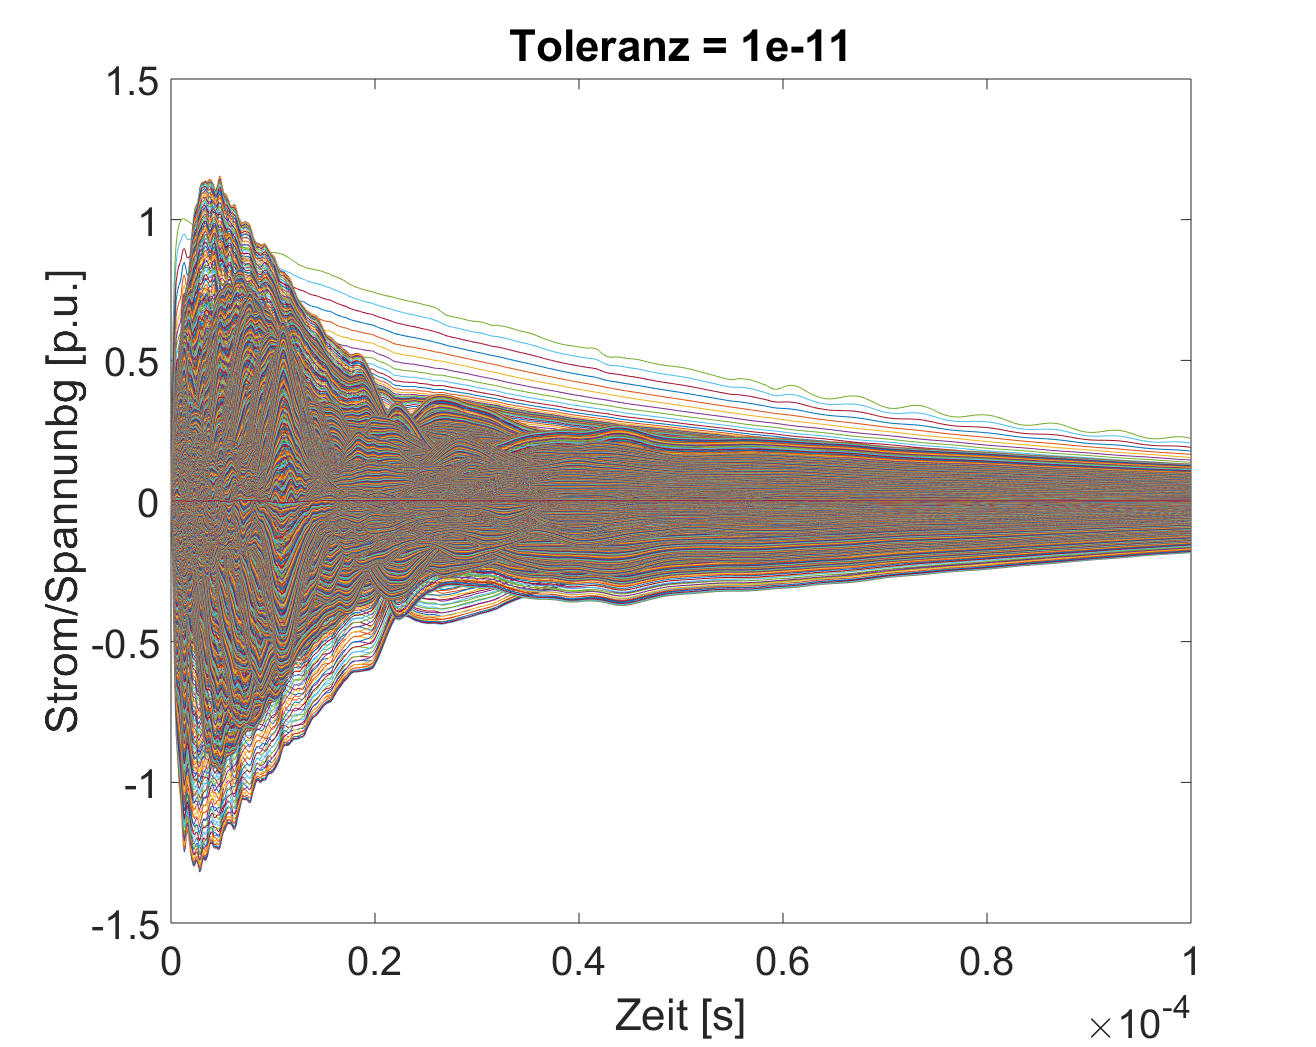
\includegraphics[width=0.7\linewidth]{./trafo/images/svd11.png}
	    \end{minipage}%
	    \begin{minipage}{.5\textwidth}
	        \centering
	        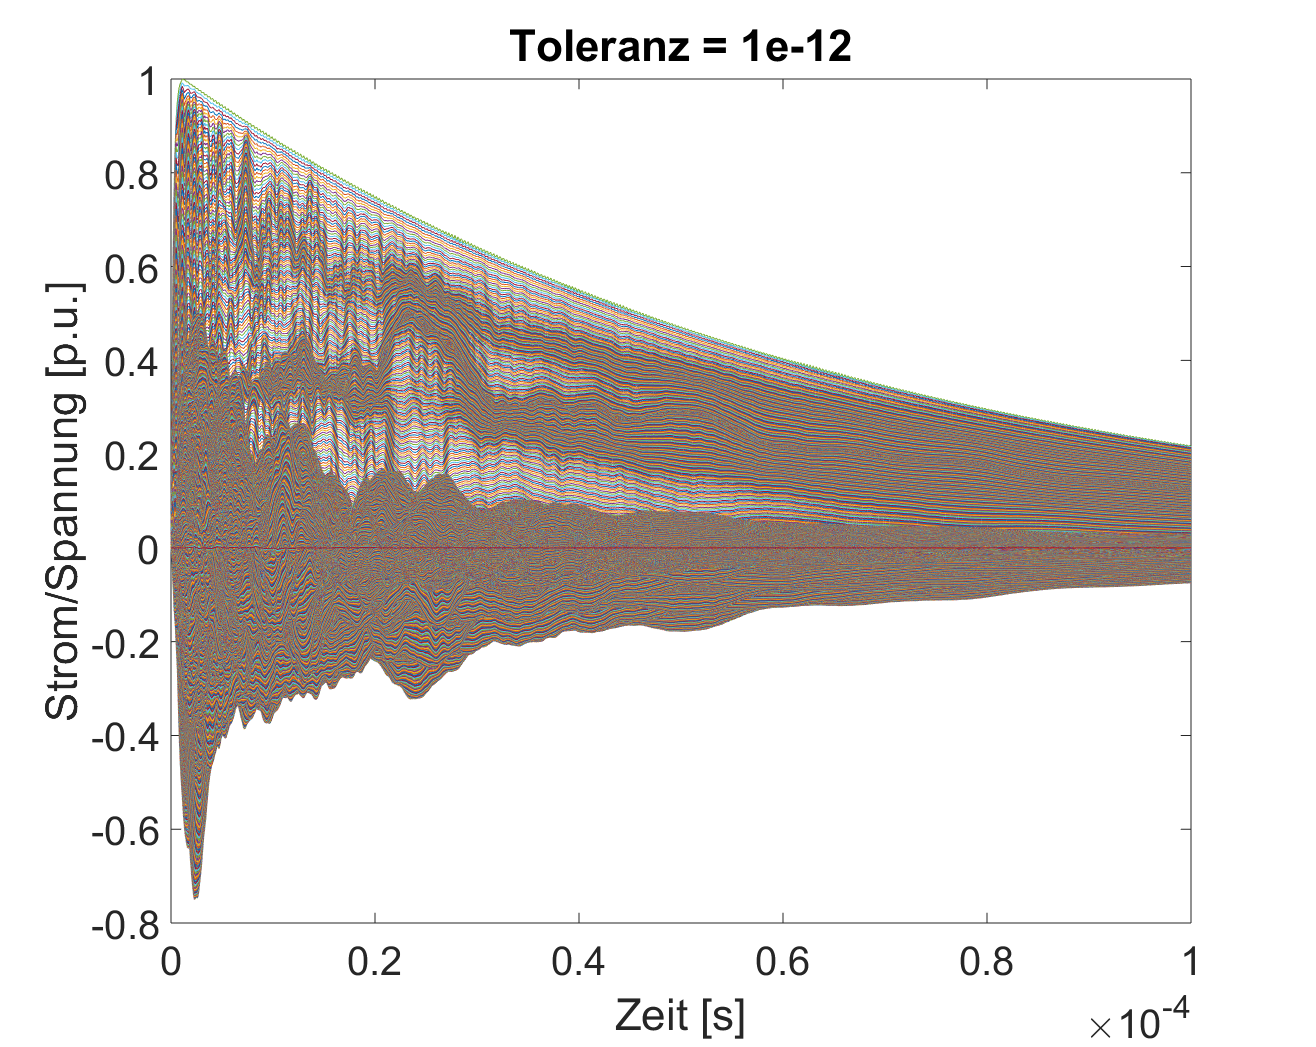
\includegraphics[width=0.7\linewidth]{./trafo/images/svd12.png}
	    \end{minipage}
		\begin{minipage}{.5\textwidth}
	        \centering
	        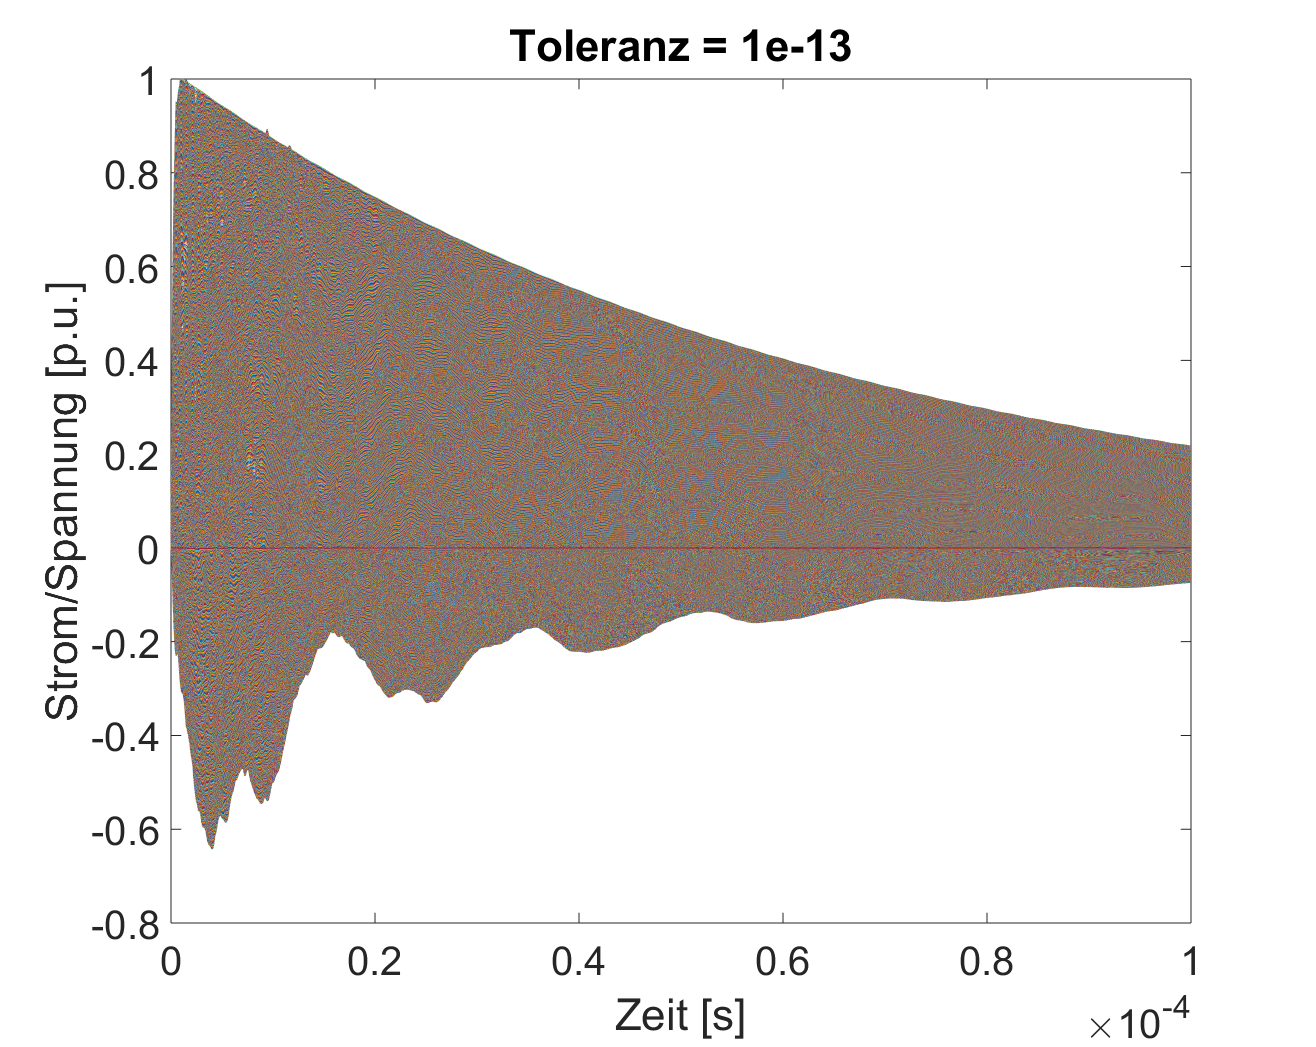
\includegraphics[width=0.7\linewidth]{./trafo/images/svd13.png}
	    \end{minipage}%
	    \begin{minipage}{.5\textwidth}
	        \centering
	        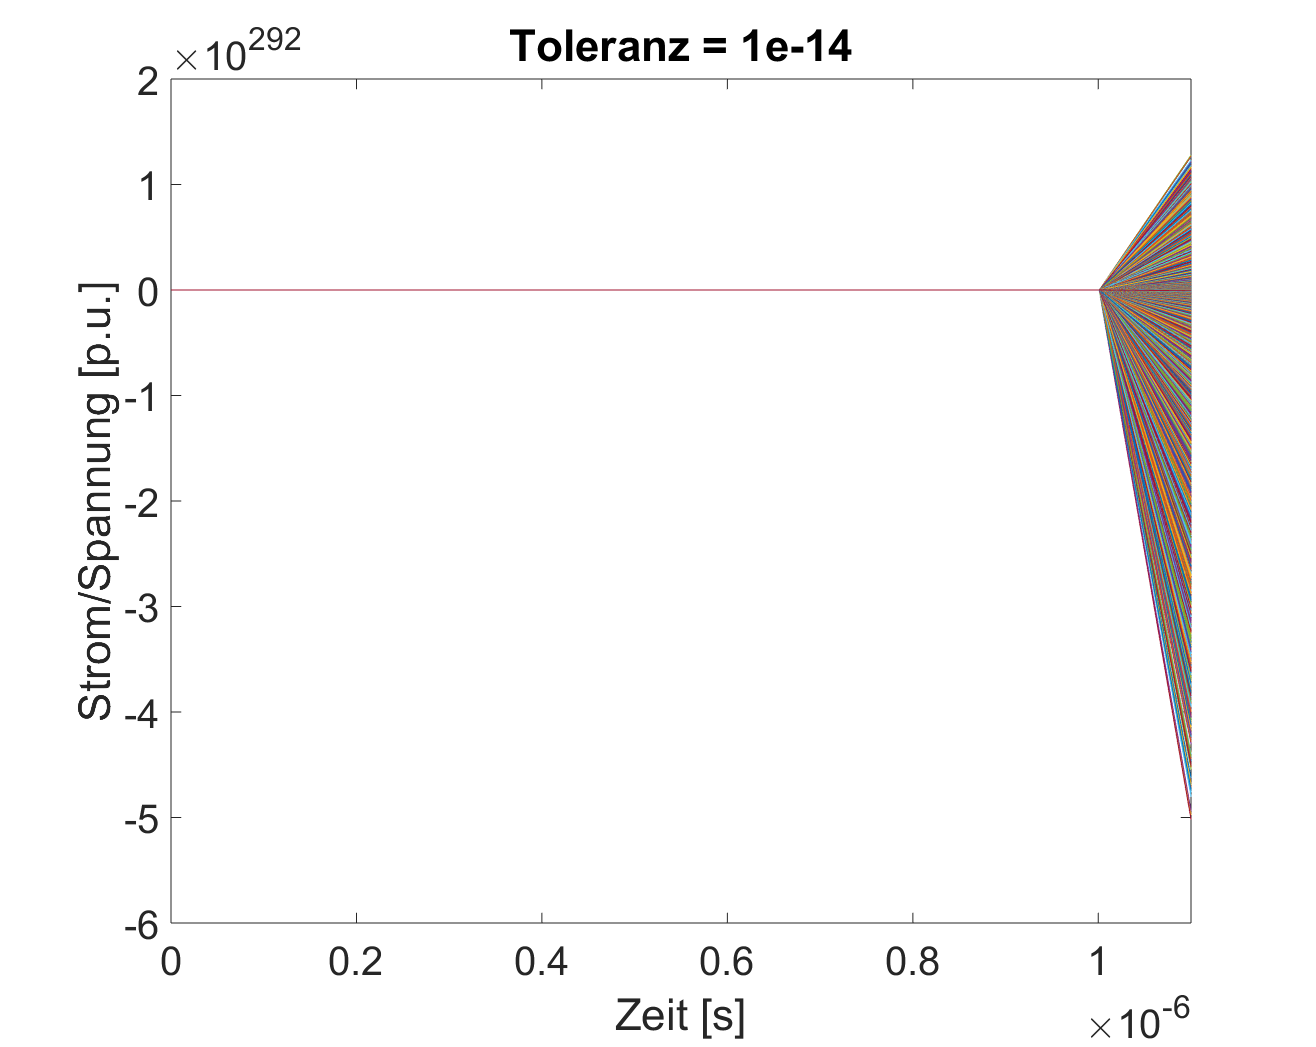
\includegraphics[width=0.7\linewidth]{./trafo/images/svd14.png}
	    \end{minipage}
	    \caption{Numerische Berechnungen mit verschiedenen Toleranzen. }
	    \label{trafo:SVDTol}
	\end{figure}

\subsection{Exaktes L"osungsverfahren}

\subsection{Schrittweite und Fehlerterm}

\subsection{Optimierungen}

Ein wichtiger Punkt bei L"osungsverfahren ist die Optimierung. Einen grossen Optimierungsschritt ist bereits beim Übergang von der $ode45$- zur exakten L"osung passiert. Es kann jedoch immer noch etwas mehr gemach werden. 

Der wesentliche Teil der Berechnung, welche beeinflusst werden kann, ist die \textit{for}-Schleife. Diese wird so viel mal durchlaufen, wie es Schritte hat. Deshalb soll das Ziel sein, m"oglichst wenig in dieser Schleife zu berechnen. 

\subsubsection{Exponentialfunktion der Eigenwerte}
Die Gleichung \ref{trafo:exakteLoesung} besitzt eine Konstante $e^{-\Lambda \cdot \Delta t}$, welche bei jedem Zeitschritt mit der neuen Anfangswerten multipliziert wird. Es macht also Sinn, diese Konstante einmal vor der Schleife zu berechnen und als Variable abzuspeichern. Da es sich bei der Matrix $\Lambda$ um eine Diagonalmatrix handelt, h"alt sich auch der Speicherbedarf der Konstante in Grenzen (es sind dies $2n + 1$ Variablen). 

\subsubsection{Lineare Interpolation}
Die soeben vorgestellte lineare Interpolation \ref{trafo:linInterp} kann mittels Umformungen in die Darstellung 

\begin{equation*}
	y_1 = y_0 \cdot e^{\lambda \cdot \Delta t} + f_0 \underbrace{\left(\left(\frac{e^{\lambda \cdot \Delta t}}{\lambda} - \frac{e^{\lambda \cdot \Delta t}}{\Delta t \cdot \lambda ^2}\right) + \frac{1}{\Delta t \cdot \lambda^2}\right)}_{a_0} + f_1 \underbrace{\left(\frac{e^{\lambda \cdot \Delta t}}{\Delta t \cdot \lambda^2} - \frac{1}{\lambda} - \frac{1}{\Delta t \cdot \lambda^2}\right)}_{a_1}
\end{equation*} 

gebracht werden. Die Konstanten $a_0$ und $a_1$ k"onnen wiederum vor der Schleife einmal berechnet werden. 

Die lineare Interpolation kann jetzt als 
\begin{equation*}
	y_1 = y_0 \cdot e^{\lambda \cdot \Delta t} + a_0 \cdot f_0 + a_1 \cdot f_1
\end{equation*}
geschrieben werden. 

Da sich bei diesem Problem nur die Eingangspannung "andert, ist die Ver"anderung vom transformiertem Vektor $f_0$ zu $f_1$ f"ur alle Elemente die selbe Zahl $f$. Die Interpolation kann noch etwas einfacher als
\begin{equation*}
	y_1 = y_0 \cdot e^{\lambda \cdot \Delta t} + (a_0 + f \cdot  a_1) \cdot f_0
\end{equation*}
geschrieben werden, wenn $f$ die Differenz der zwei Vektoren $f_0$ und $f_1$ ist. 

\subsubsection{Implementation}
Der Matlab-Code kann jetzt folgendermassen geschrieben werden.

{\scriptsize \lstinputlisting{./trafo/code/compact.m}}

\subsubsection{Vergleich}

Um die Performance zu testen, wird eine sehr schlechte Implementation gew"ahlt, welche eine lineare Interpolation besitzt. Im Gegensatz zum soeben gezeigten Code werden in dieser schlechten Variante allerdings alle Konstante in der \textit{for}-Schleife berechnet. Jeder einzelner Zeitschritt dauert in der Berechnung ca. \SI{130}{\milli\second}. 

Als Vergleich wird die schnellste Optimierung verwendet (Matlab-Code von oben). Die Berechnungszeit f"ur jeden einzelnen Zeitschritt konnte bis auf \SI{35}{\micro \second} reduziert werden. 

Die Grafik \ref{trafo:Optimierung} zeigt den Unterschied in einer doppelt logarithmischen Grafik. Die Optimierungsversuche haben sich auch in der Praxis als hervorragend erwiesen.

\begin{figure}
	\centering
	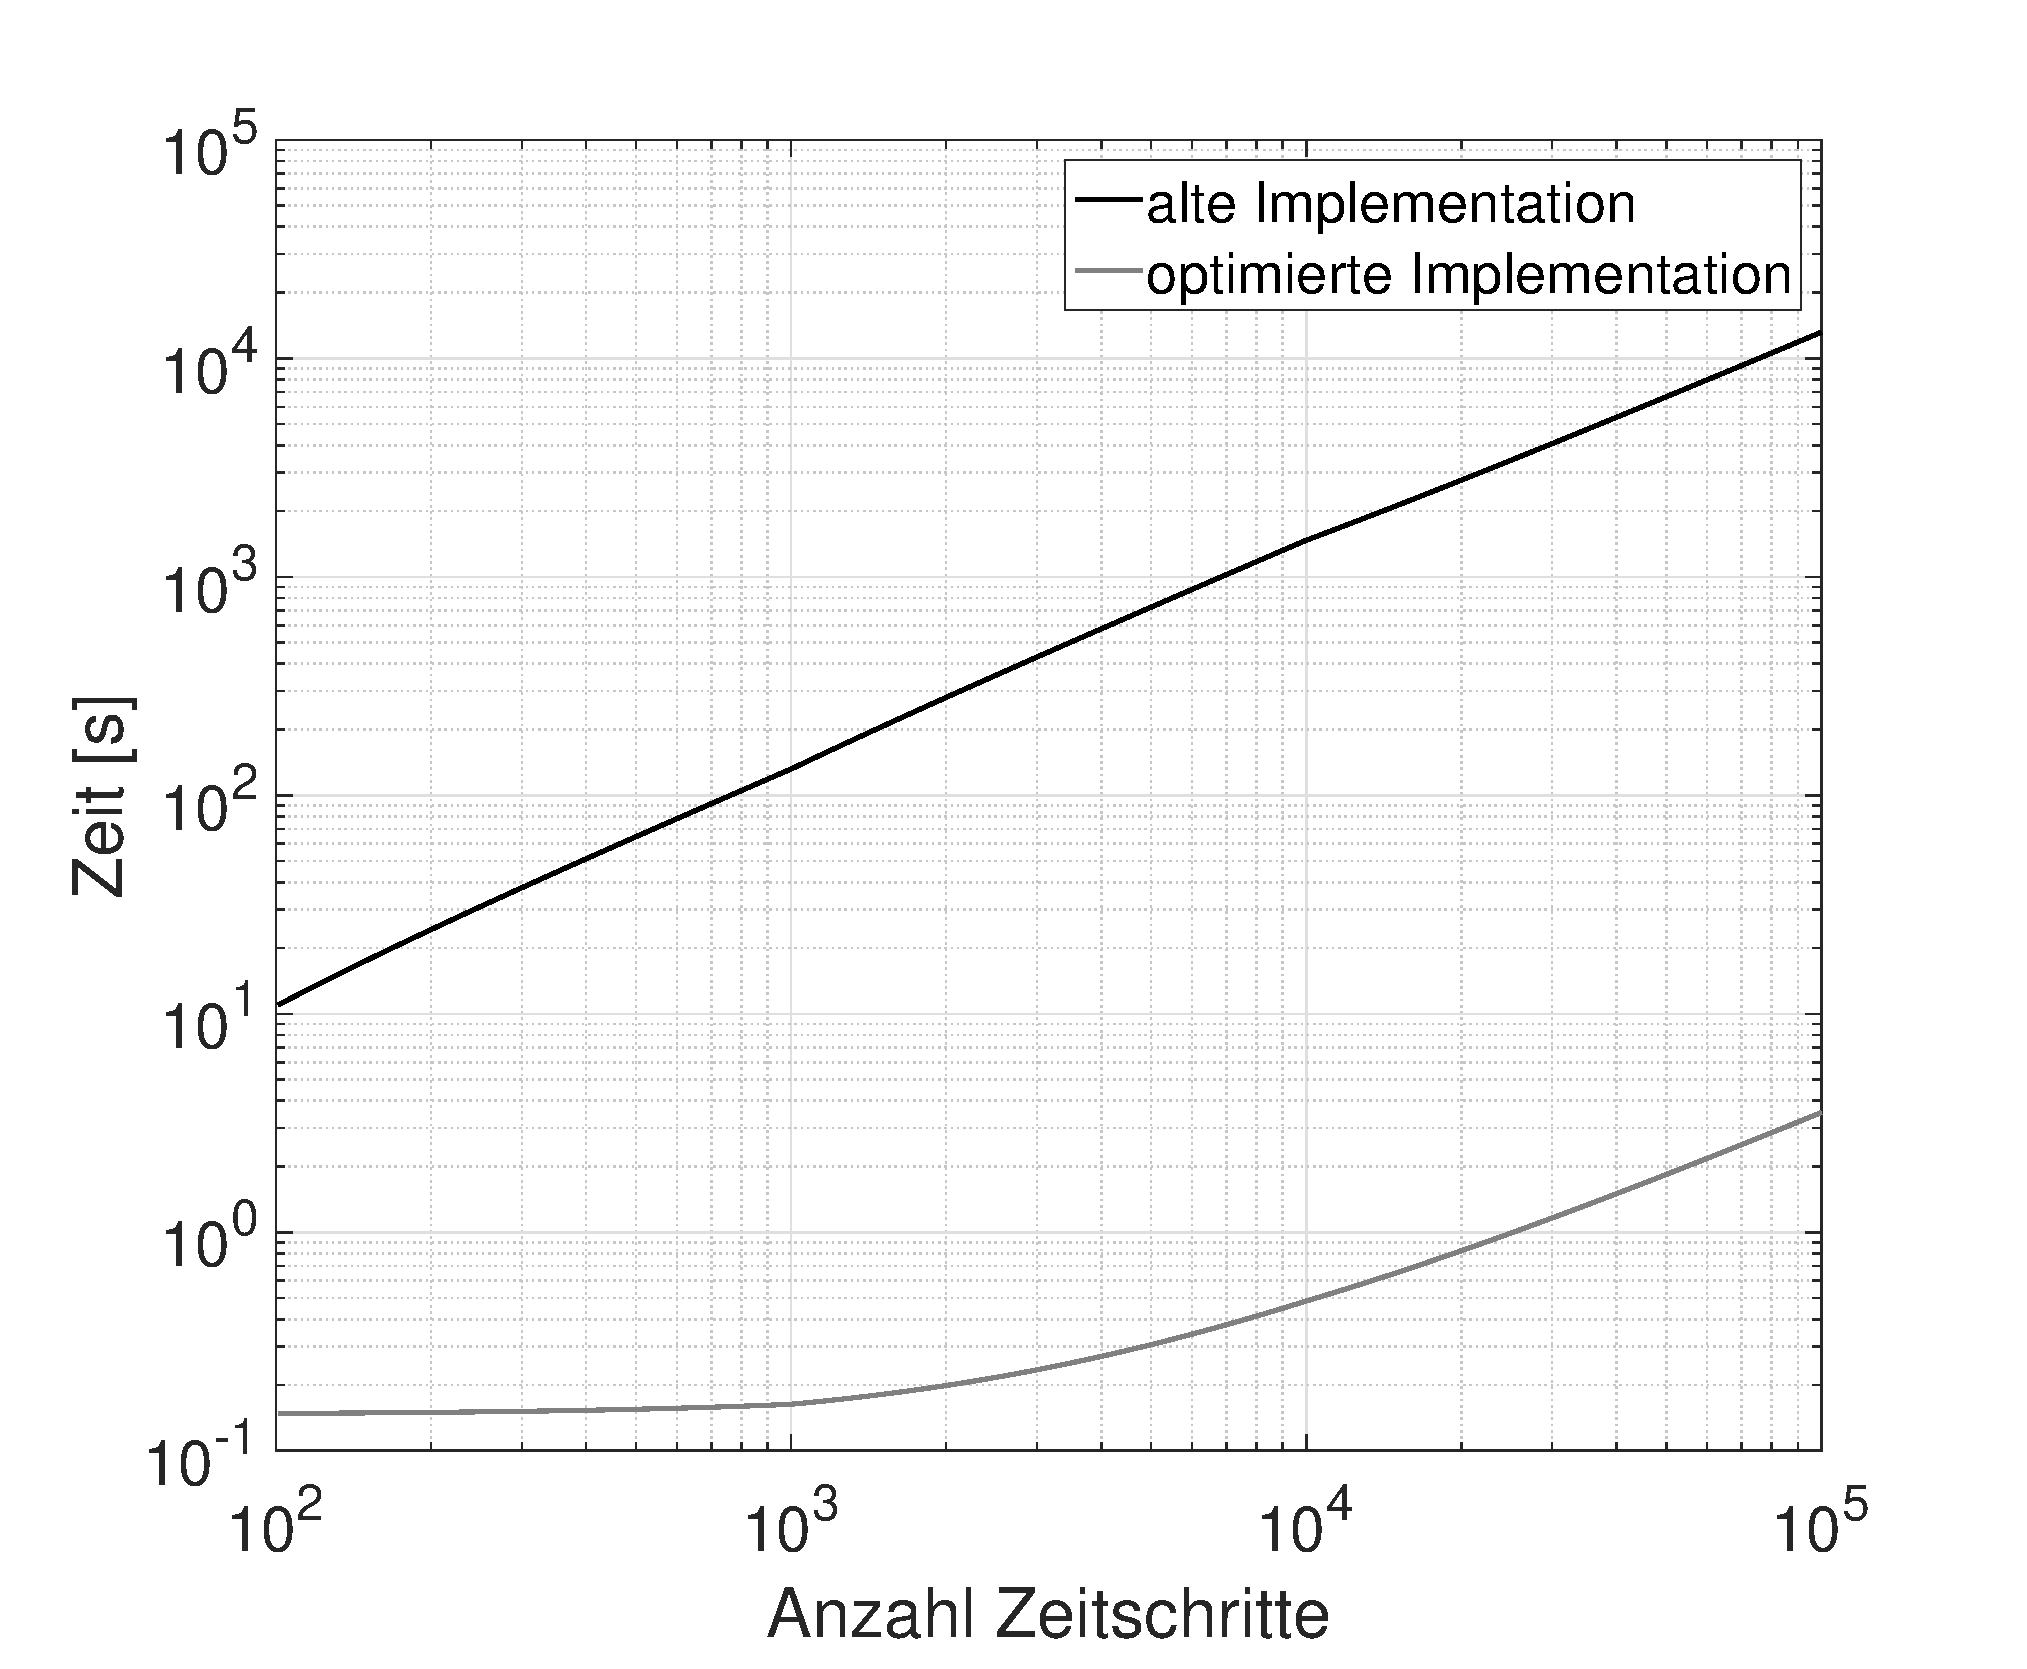
\includegraphics[width=0.8\textwidth]{./trafo/images/differenceOptimization.eps}
	\caption{Unterschied zwischen einer sehr schlechten und einer guter Implementierung.}
	\label{trafo:Optimierung}
\end{figure}

\section{Anwendung der gefundenen L"osungen}

Schlussendlich k"onnen die gefundenen L"osungen wieder in das CAD-Modell eingelesen werden, damit das elektrische Feld simuliert werden kann. Somit kann festgestellt werden, wo sich Schwachstellen im Transformator befinden und allenfalls verbessert werden.

Interessant ist nat"urlich immer der gr"osste Spannungsunterschied zwischen benachbarten Wicklungen. In diesem Beispiel ist dies zwischen dem Layer 1 und 2 zwischen Wicklung 6 und 118.

Diese L"osung wurde bereits in Abbildung \ref{trafo:loesung} pr"asentiert. Das elektrische Feld beim Zeitpunkt der gr"ossten Spannungsdifferenz ist in Abbildung \ref{trafo:E-Field} und \ref{trafo:E-FieldZoom} dargestellt. 

\begin{figure}
	\centering
	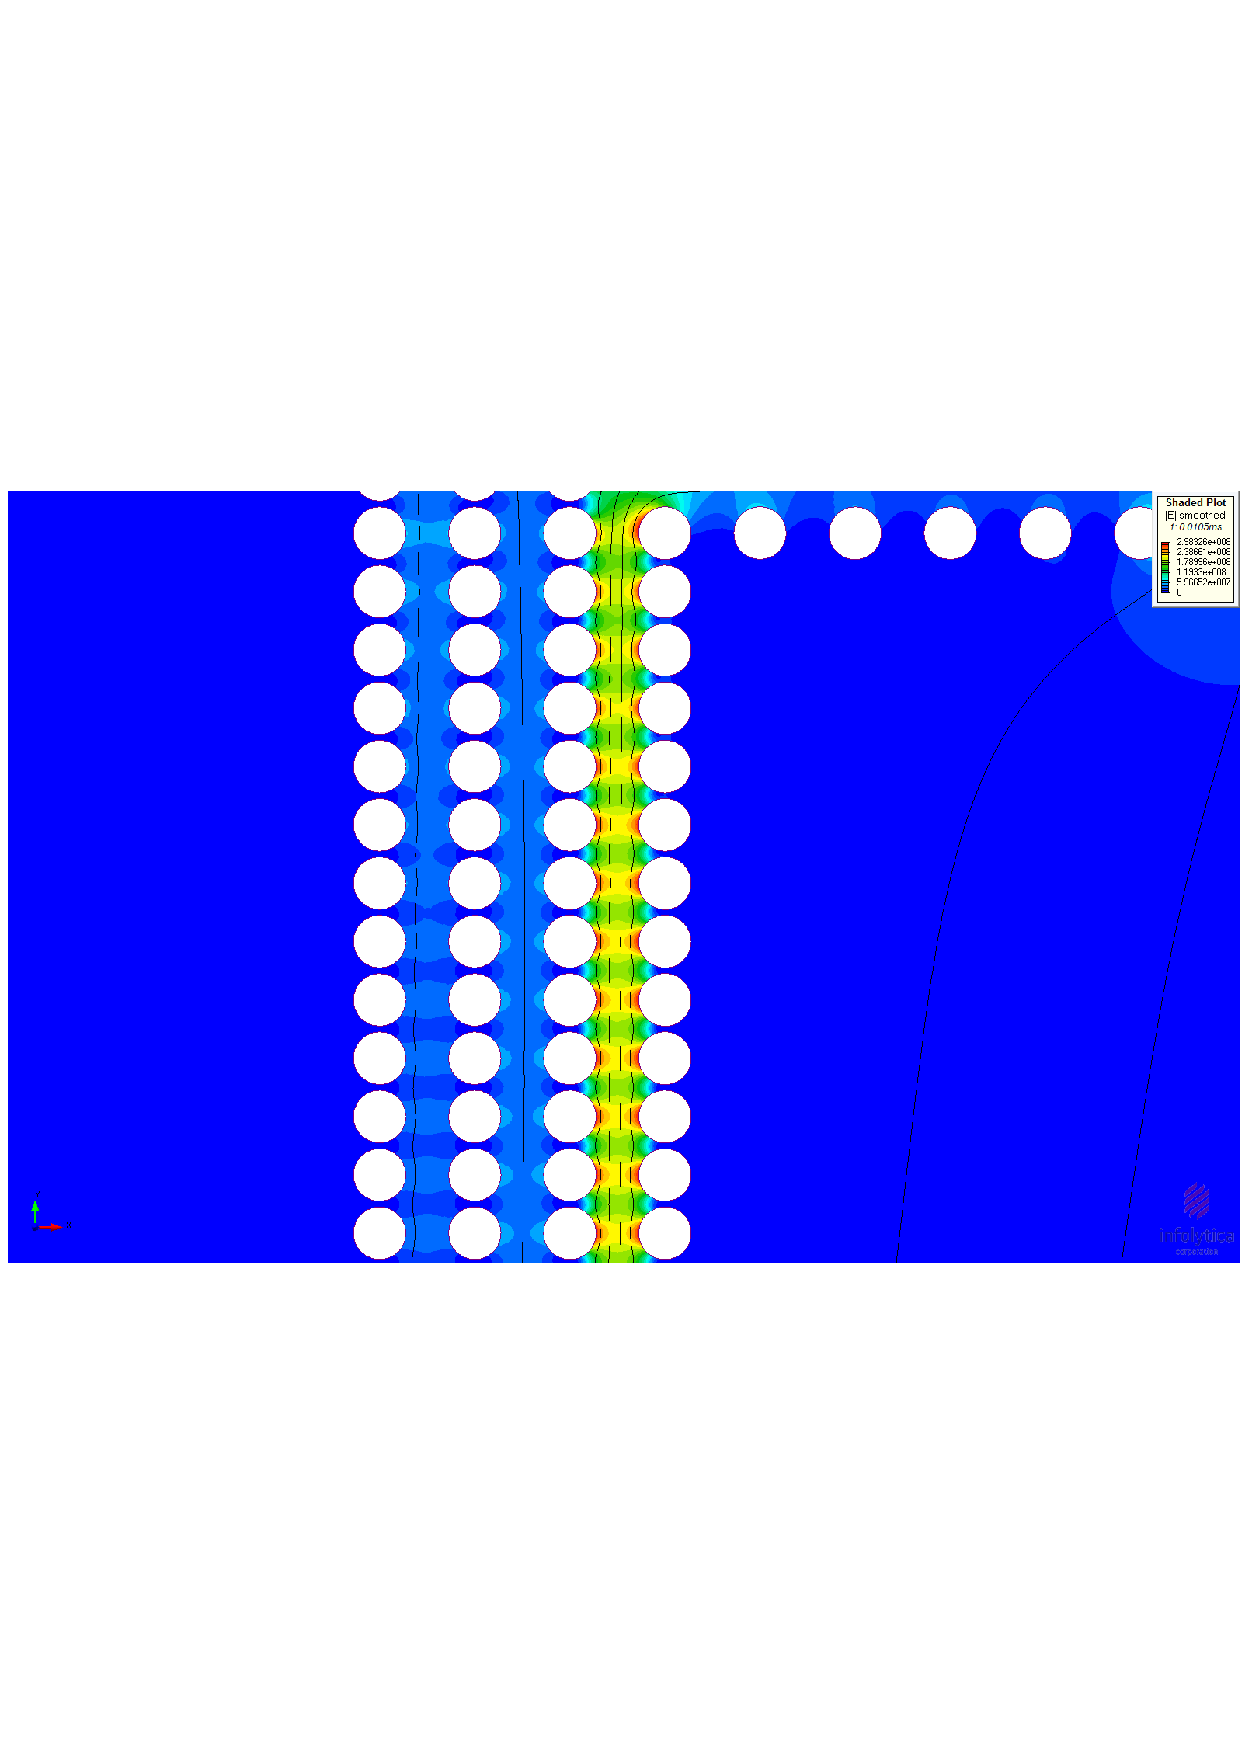
\includegraphics[width=\textwidth]{./trafo/images/BIL_VoltageTrans.pdf}
	\caption{Elektrisches Feld zwischen den ersten paar Layern.}
	\label{trafo:E-Field}
\end{figure}

\begin{figure}
	\centering
	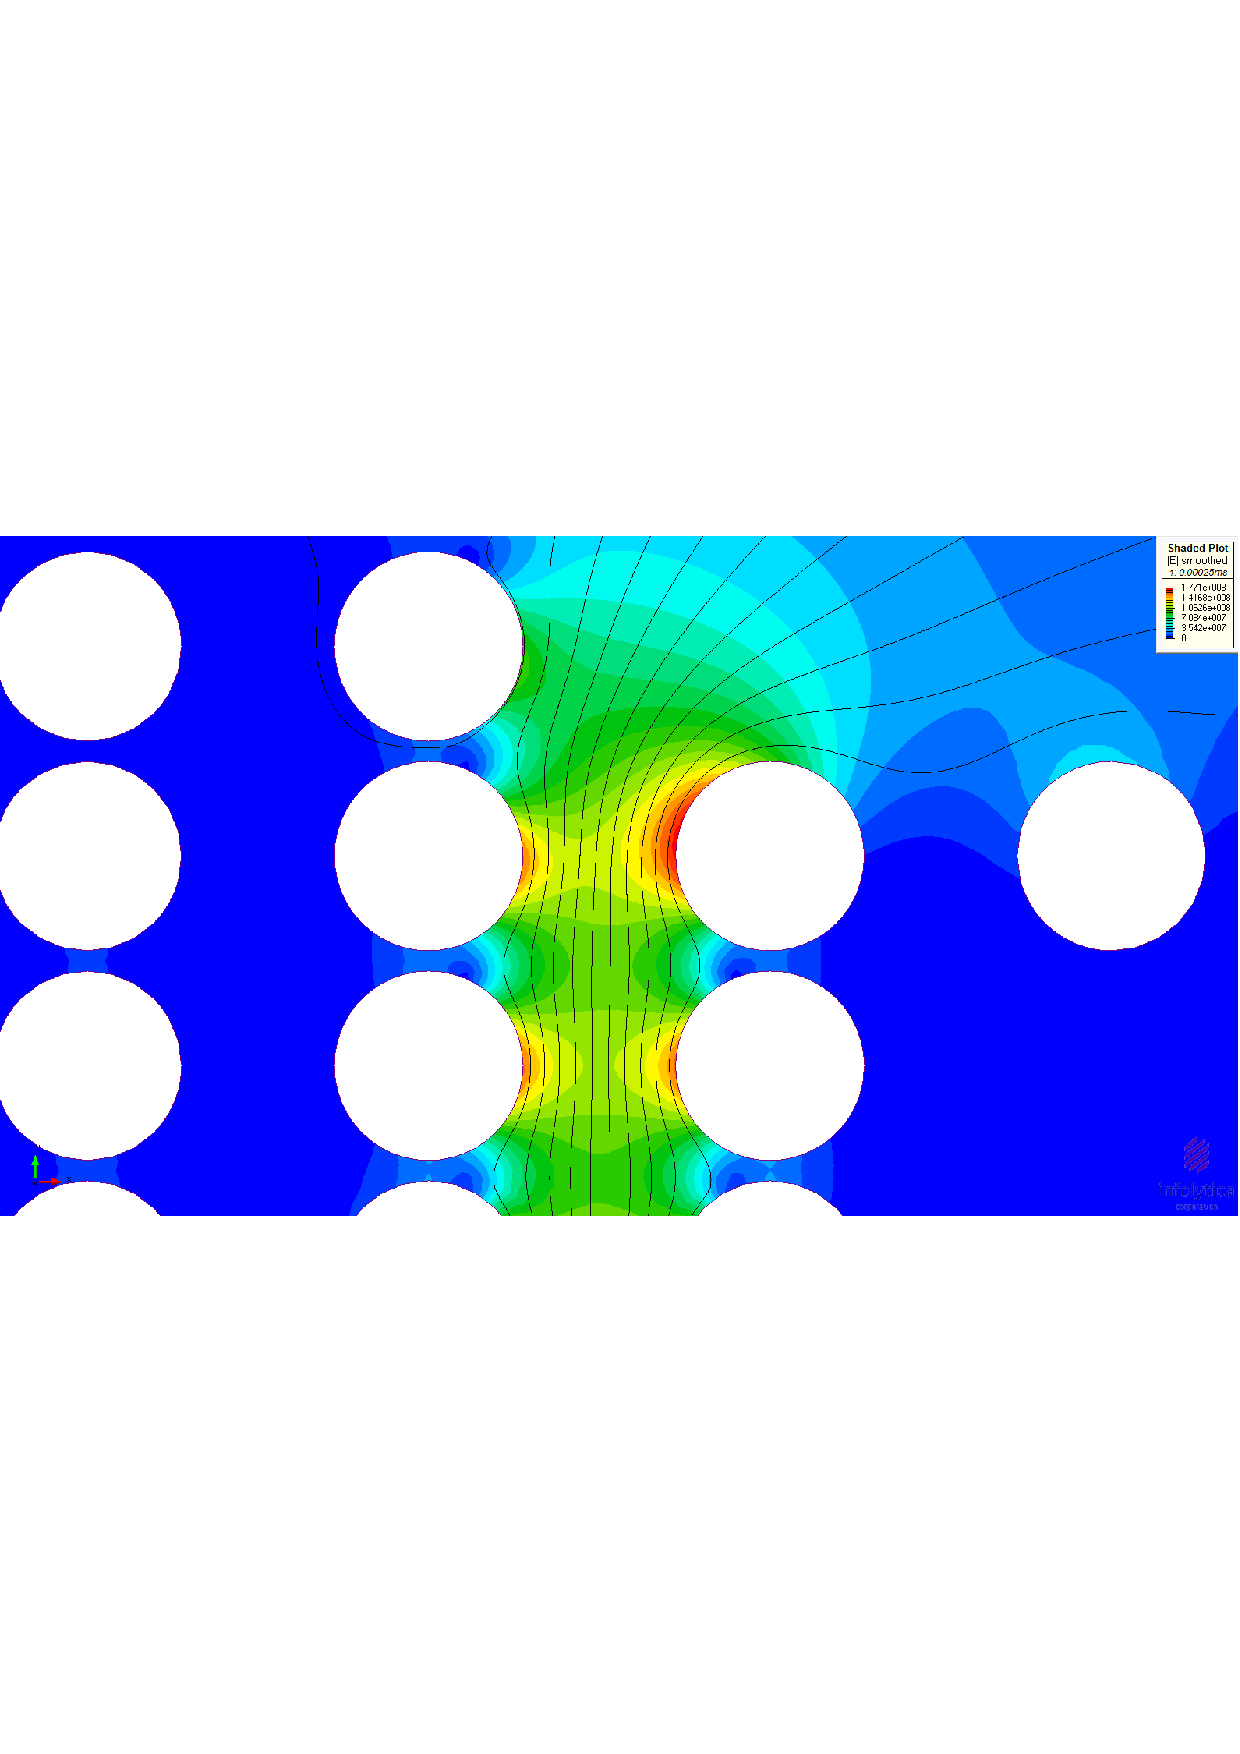
\includegraphics[width=\textwidth]{./trafo/images/VoltageTrans.pdf}
	\caption{Elektrisches Feld zwischen Windung 6 und 118.}
	\label{trafo:E-FieldZoom}
\end{figure}

Da die Herstellung von Transformatoren nie optimal ablaufen, k"onnen sich auch Luftblasen im Epoxidharz bilden. Diese Luftblasen, auch Lunker genannt, verst"arken das elektrische Feld zus"atzlich und schw"achen somit den Transformator im Fehlerfall. Ein m"ogliches Szenario ist in Abbildung \ref{trafo:E-FieldBubble} pr"asentiert. 

\begin{figure}
	\centering
	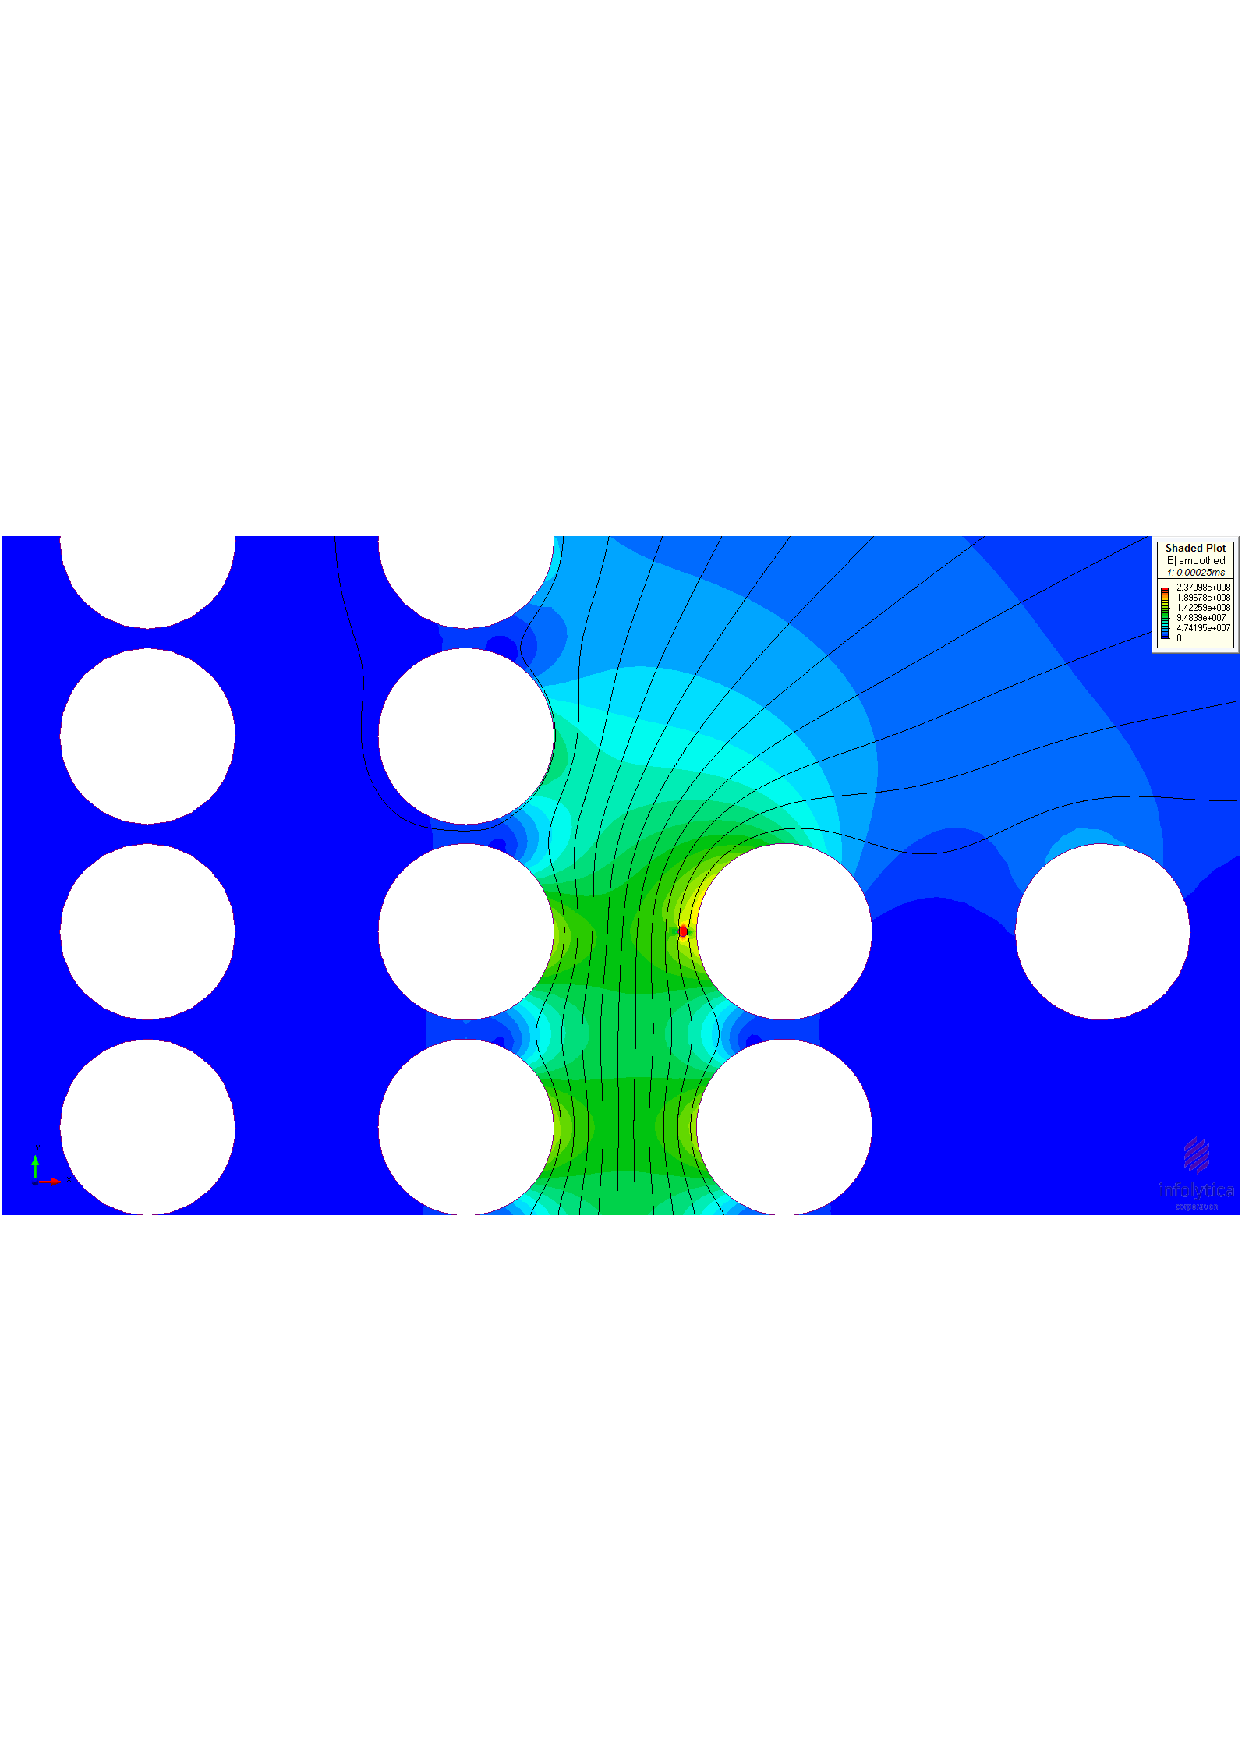
\includegraphics[width=\textwidth]{./trafo/images/VoltageTrans_bubble_turn6_10u_9u.pdf}
	\caption{Elektrische Feld zwischen Wicklung 6 und 118 mit simulierter Luftblase (Lunker).}
	\label{trafo:E-FieldBubble}
\end{figure}

\subsection{Schlussfolgerung}
Das Problem kann erfolgreich formuliert werden und automatisiert werden. Mit mathematischen Hilfsmitteln ist es auch m"oglich grosse Matrizen zu berechnen.

\printbibliography[heading=subbibliography]
\end{refsection}
